% !TEX root = ../thesis.tex
\chapter{Introduction}
\label{ch:intro}

\section{Spatial regression with partial differential equation regularization}
This work naturally stems from the studies in the research field called
\textit{spatial regression with partial differential equation regularization},
abbreviated in the following as SR-PDE. SR-PDE constitutes a family of models
which has been, and still is, under study beginning from \citeyear{sangalli0}
in \citeauthor{sangalli0} \cite{sangalli0}.

SR-PDE effectively combines several branches of mathematics and statistics
modeling. For a thorough analysis of its derivation and the enhancements it
brings to the existing literature see \cite{sangalli1}, I will limit myself to
a brief introduction.\\ SR-PDE models feature the minimization of a functional
composed of two terms: a classical least-square term, with the goal of
estimating a vector of unknown regression coefficients (in case of presence of
covariates), and a regularization term, estimating an unknown deterministic
spatial field.\\ The spatial field contributes to the functional by integration
over the spatial domain of the square of a differential operator, most commonly
the Laplacian operator. By properties of the Laplace operator, this choice
induces an isotropic and stationary smoothing effect on the unknown spatial
field, meaning equal in every direction and independent on the position. Other
differential operators considered in this work are generic second order
differential operators, that come from the physics of the problem or from some
preexisting knowledge about the phenomenon under study.

The inclusion of partial differential equations in the statistical model brings
many advantages, like the aforementioned ability to include problem-specific
knowledge, dealing with boundary conditions, etc., but makes computations more
cumbersome.

\section{Mixed-effects models}
In a situation where observed data possess a natural grouping structure,
mixed-effects models are often utilized. They combine fixed effects, meaning
that a set of covariates have regression coefficients shared among all groups,
and random effects, meaning the remaining set of covariates have regression
coefficients varying along each group.

Given our interest in spatial data analysis, a typical situation in which
mixed-models are used is in clinical data, where data of several patients are
measured in the same area of the body. For example in chapter
\ref{ch:Applications} \nameref{ch:Applications}, we will see a mixed-effects
model applied to human brain data, collected on a set of patients who undertook
functional Magnetic Resonance Imaging (fMRI).\\ We will denote as statistical
unit the entity being observed that induces the grouping structure: in the just
mentioned clinical example, the statistical units are the different patients
being observed.

We are therefore ready to present, similarly as in \cite{kim}, the SR-PDE
mixed-effects model.

\section{Generic SR-PDE mixed-effects model}

Consider $m$ statistical units. To the $i$-th unit, with $i$ varying from 1 to
m, corresponds a unique spatial domain $\Omega_i$, on which we observe $n_i$
data at different positions $\bm{p}_{ij}$. Index $j$ is therefore varying from
$1$ to $n_i$, for given statistical unit $i$.\\The variable of interest z,
observed at $\bm{p}_{ij}$, is modeled as
\begin{equation}
	\label{model}
	z_{ij} = \bm{w}^T_{ij} \bm{\beta} + \bm{v}^T_{ij} \bm{b}_i + f_i(\bm{p_}{ij}) + \epsilon_{ij}.
\end{equation}
The notation used represents the following quantities:
\begin{itemize}
	\item[--] $\bm{w}_{ij}$ is the vector of fixed effects covariates for the
		observation $z_{ij}$; \item[--] $\bm{\beta}$ is the vector of regression
		coefficients for fixed effects; \item[--] $\bm{v}_{ij}$ is the vector of random
		effects covariates for the observation $z_{ij}$; \item[--] $\bm{b}_i$ is the
		vector of regression coefficients of the random effects for unit $i$; \item[--]
		$f_i$ is the unknown deterministic field defined on domain $\Omega_i$;
	\item[--] $\epsilon_{ij}$, for every $i$ and $j$, are the random noise or
		errors, considered as the realizations of independent identically distributed
		(i.i.d.) random variables, with mean $0$ and variance $\sigma^2$.
\end{itemize}
We will assume that the random effect $\bm{b}_i$ has average $0$
\begin{equation}
	\label{constraint}
	\sum_{i=1}^{m}{\bm{b}_i}=0.
\end{equation}
In fact, if the average was different from 0, we would simply split
the contribution of those covariates into two, a fixed effect one and a random
effect covariate with 0 average across groups (more on this in section
\ref{repar}, \nameref{repar}). \\ Let also $N$ be equal to $\sum_{i=1}^{m}n_i$.
For every $i$, $j$ equation \ref{model} constitutes a system of $N$ equations,
that is expressed concisely in algebraic form in the following two ways:
\begin{equation}
	\begin{cases}
		\bm{z}_i = W_i \bm{\beta} + V_i \bm{b}_i + \bm{f_i} + \bm{\epsilon_i} \qquad
		i=1\dots m \\
		\sum_{i=1}^{m}{\bm{b}_i}=0
	\end{cases}
\end{equation}
and
\begin{equation}
	\label{unconstrained}
	\bm{z} = W \bm{\beta} + V \bm{b} + \bm{f}_N + \bm\epsilon,
\end{equation}
in which the corresponding terms in the two equations have the
following meanings:
\begin{itemize}
	%	\item[--]
	%		\listvalues
	\item[--] $\bm{z}_i \in \R^{n_i}$ is the vector of observed data for unit $i$
		and $\bm{z}$ is the vector belonging to $\R^N$ obtained by concatenating the
		$m$ vectors $\bm{z}_i$;
	\item[--] $W_i$ is the matrix whose element $w_{j,k}$
		is the $k$-th element of previously defined vector $\bm{w}_{ij}$,
		$\left(\bm{w}_{ij}\right)_k$, whereas $W$ is a concatenation as well
		\begin{equation}
			W=
			\begin{bmatrix*}
				W_1\\
				\vdots\\
				W_m
			\end{bmatrix*}
			;
		\end{equation}
	\item[--] $V_i$ is the matrix whose element $v_{j,k}$ is the $k$-th
		element of previously defined vector $\bm{v}_{ij}$,
		$\left(\bm{v}_{ij}\right)_k$;
	\item[--] when moving to the $N$ system of
		equations, we include constraint \ref{constraint} by defining $\bm{b}$ as the
		concatenation of $m-1$ vectors $\bm{b}_i$, omitting the last one
		\begin{equation}
			\bm{b}=
			\begin{bmatrix*}
				\bm{b}_1\\
				\vdots\\
				\bm{b}_{m-1}
			\end{bmatrix*}
		\end{equation}
		and defining $V$ in the following manner:
		\begin{equation}
			V=
			\begin{bmatrix*}
				V_1 & 0 & 0 & 0\\
				0 & V_2 & 0 & 0\\
				\vdots & 0 & \ddots & \vdots\\
				0 & 0 & 0 & V_{m-1}\\
				-V_m & -V_m & -V_m & -V_m
			\end{bmatrix*}
			;
		\end{equation}
	\item[--] $\bm{f}_i \in \R^{n_i}$ is the vector of observed data for
		unit $i$ and $\bm{f}_N$ is the vector belonging to $\R^N$ obtained by
		concatenating the $m$ vectors $\bm{f}_i$;
	\item[--] $\bm{\epsilon}_i \in
			\R^{n_i}$ is the vector of errors for unit $i$ and $\bm{\epsilon}_N$ is the
		vector belonging to $\R^N$ obtained by concatenating the $m$ vectors
		$\bm{\epsilon}_i$.
\end{itemize}
\section{Reparametrizing the model}\label{repar}
The $N$ system of equations \ref{unconstrained} is the model written in an
unconstrained form, where the constraint \ref{constraint} has been “injected”
into the design matrix. We also call it \textit{official parametrization} of
the mixed-effects model.

As described in \cite{kim} we prefer to adopt a slightly different approach,
mainly for computational efficiency reasons. In the following we will assume
that all covariates contribute to the fixed effect part of the model, whereas a
subset of them will contribute to the random effect part. We will refer to this
version of the model as the \textit{implementation} one.

\textit{Implementation} version is expressed by the following system:
\begin{equation}
	\bm{z}=W' \bm{\beta}' +V'\bm{b}' +\bm{f}_N + \bm{\epsilon},
\end{equation}
where we have used the following new quantities:
\begin{itemize}
	\item[--] $W'$, similarly as before, is concatenation of $W_i'$ matrices, where
		$W_i'$ is composed of the covariates related only to fixed effects, meaning
		with no unit-specific contribution.
		\begin{equation}
			W'=
			\begin{bmatrix*}
				W_1'\\
				W_2'\\
				\vdots\\
				W'_{m}
			\end{bmatrix*}
			;
		\end{equation}
	\item[--] $\bm{\beta}'$ is the coefficient relative to covariates for
		fixed effects, as just described; \item[--] $V'$ is composed of $V_i'$
		matrices, which are the matrices of covariates having also a random effect.
		Unlike previous $V$, $V'$ does not include the part deriving from constraint
		\ref{constraint}:
		\begin{equation}
			V'=
			\begin{bmatrix*}
				V_1' & 0 & 0 & 0\\
				0 & V_2' & 0 & 0\\
				\vdots & 0 & \ddots & \vdots\\
				0 & 0 & 0 & V_{m}'
			\end{bmatrix*}
			;
		\end{equation}
	\item[--] $\bm{b}'$ is the regression coefficient relative to the
		covariates with unit-specific effect,
		\begin{equation}
			\bm{b}'=
			\begin{bmatrix*}
				\bm{b}'_1\\
				\vdots\\
				\bm{b}'_{m}
			\end{bmatrix*}
			;
		\end{equation}
\end{itemize}
To properly refer to sizes of vectors and matrices defined before, we
use the following notation. We indicate with $q$ the number of covariates, and
with $p$ the number of covariates with unit-specific interest. Therefore $q-p$
is the number of covariates considered for their fixed effect contribution
only.

Vector $\bm{b}'$ belongs to $\R^{mp}$, $\bm{\beta}'$ to $\R^{q-p}$ and we can
relate it to previously defined vectors $\bm{b}$, $\bm{\beta}$ ($\in
	\R^{m(p-1)},\R^q$ respectively), by defining $\bm{\beta}^* \in \R^p$, average
of random effects coefficients
\begin{equation}
	\bm{\beta}^*=\frac{\sum_{i=1}^{m}\bm{b}'_i}{m}.
\end{equation}
In this way $\bm{\beta}$ is just the concatenation of $\bm{\beta}'$
and $\bm{\beta}^*$ while for $\bm{b}$ holds the following:
\begin{equation}
	\bm{b}=
	\begin{bmatrix}
		\bm{b}_1 \\
		\bm{b}_2 \\
		\vdots   \\
		\bm{b}_{m-1}
	\end{bmatrix}
	=
	\begin{bmatrix}
		\bm{b}_1' -\bm{\beta}^* \\
		\bm{b}_2' -\bm{\beta}^* \\
		\vdots                  \\
		\bm{b}_{m-1}' -\bm{\beta}^*
	\end{bmatrix}
	.
\end{equation}

For what concerns the sizes of the matrices defined before, we deduce that $W_i
	\in \R^{n_i \times q}$, $W \in \R^{N \times q}$, $V_i \in \R^{n_i \times p}$,$V
	\in \R^{N \times p}$, $W'_i \in \R^{n_i \times \left(q-p\right)}$, $W' \in
	\R^{N \times \left(q-p\right)}$, $V'_i \in \R^{n_i \times p}$,$V' \in \R^{N
		\times p}$.
\section{Estimation problem}
Similarly to what happens with every SR-PDE model, we estimate the unknown
quantities of the model by solving, with the necessary approximations, the
following minimization problem:
\begin{equation}
	\label{problem}
	\textrm{Find} \argmin_{\bm{\beta}', \bm{b}', f_1, \dots, f_m}{J_{\Omega_i, \lambda} \left(\bm{\beta}', \bm{b}', f_1, \dots, f_m \right)}
\end{equation}
where the functional $J_{\Omega_i, \lambda}$ is defined as
\begin{equation}
	\label{functional}
	J_{\Omega_i, \lambda} \left(\bm{\beta}', \bm{b}', f_1, \dots, f_m \right) =
	\norm{\bm{z}-W' \bm{\beta}' -V'\bm{b}' -\bm{f}_N}^2 + \lambda \sum_{i = 1}^m \int_{\Omega_i}\Delta f_i \left(\bm{p}\right)^2 d\Omega_i ,
\end{equation}
or equivalently, in a more lengthy expression:
\begin{multline}
	J_{\Omega_i, \lambda} \left(\bm{\beta}', \bm{b}'_1, \dots, \bm{b}'_m, f_1, \dots, f_m \right) = \\ \sum_{i = 1}^m \left( \sum_{j=1}^{n_i} \left( z_{ij}-{\bm{w}'_{ij}}^T \bm{\beta}' - {\bm{v}'_{ij}}^T \bm{b}'_i - f_i(\bm{p_{ij}}) \right)^2 + \lambda \int_{\Omega_i} \Delta f_i \left(\bm{p}\right)^2 d\Omega_i\right).
\end{multline}
For simplicity, we have considered the Laplacian as differential
operator, but more general choices are possible.

It shall be noticed that the unknown field must not satisfy the differential
equation but contributes to the functional with the square of its misfit from
the equation itself --- besides its contribution in terms of distance from
observed data.

We now introduce the notation necessary to tackle problem \ref{problem}, and
characterize the solution defined on suitable spaces. Assuming $W'_i$ and
$V'_i$ for $i=1,\dots,m$ full rank, we define the following matrices:
\begin{equation}
	\label{matrix:x}
	X =
	\begin{bmatrix}
		W'_1     & V'_1   & 0      & \ldots & 0        & 0      \\
		W'_2     & 0      & V'_2   & \ldots & 0        & 0      \\
		\vdots   & \vdots & \vdots & \ddots & \vdots   & \vdots \\
		W'_{m-1} & 0      & 0      & \ldots & V'_{m-1} & 0      \\
		W'_m     & 0      & 0      & \ldots & 0        & V'_m
	\end{bmatrix}
\end{equation}
\begin{equation}
	H = X\left(X^TX\right)^{-1}X^T
\end{equation}
\begin{equation}
	Q = I_N - H
\end{equation}
with $X\in \R^{N\times (mp+q-p)}$, H and Q $\in \R^{N\times N}$ are
the matrices that project a vector, respectively, onto the subspace spanned by
the columns of X and onto its orthogonal complement with respect to $\R^N$.
\begin{figure}[t]
	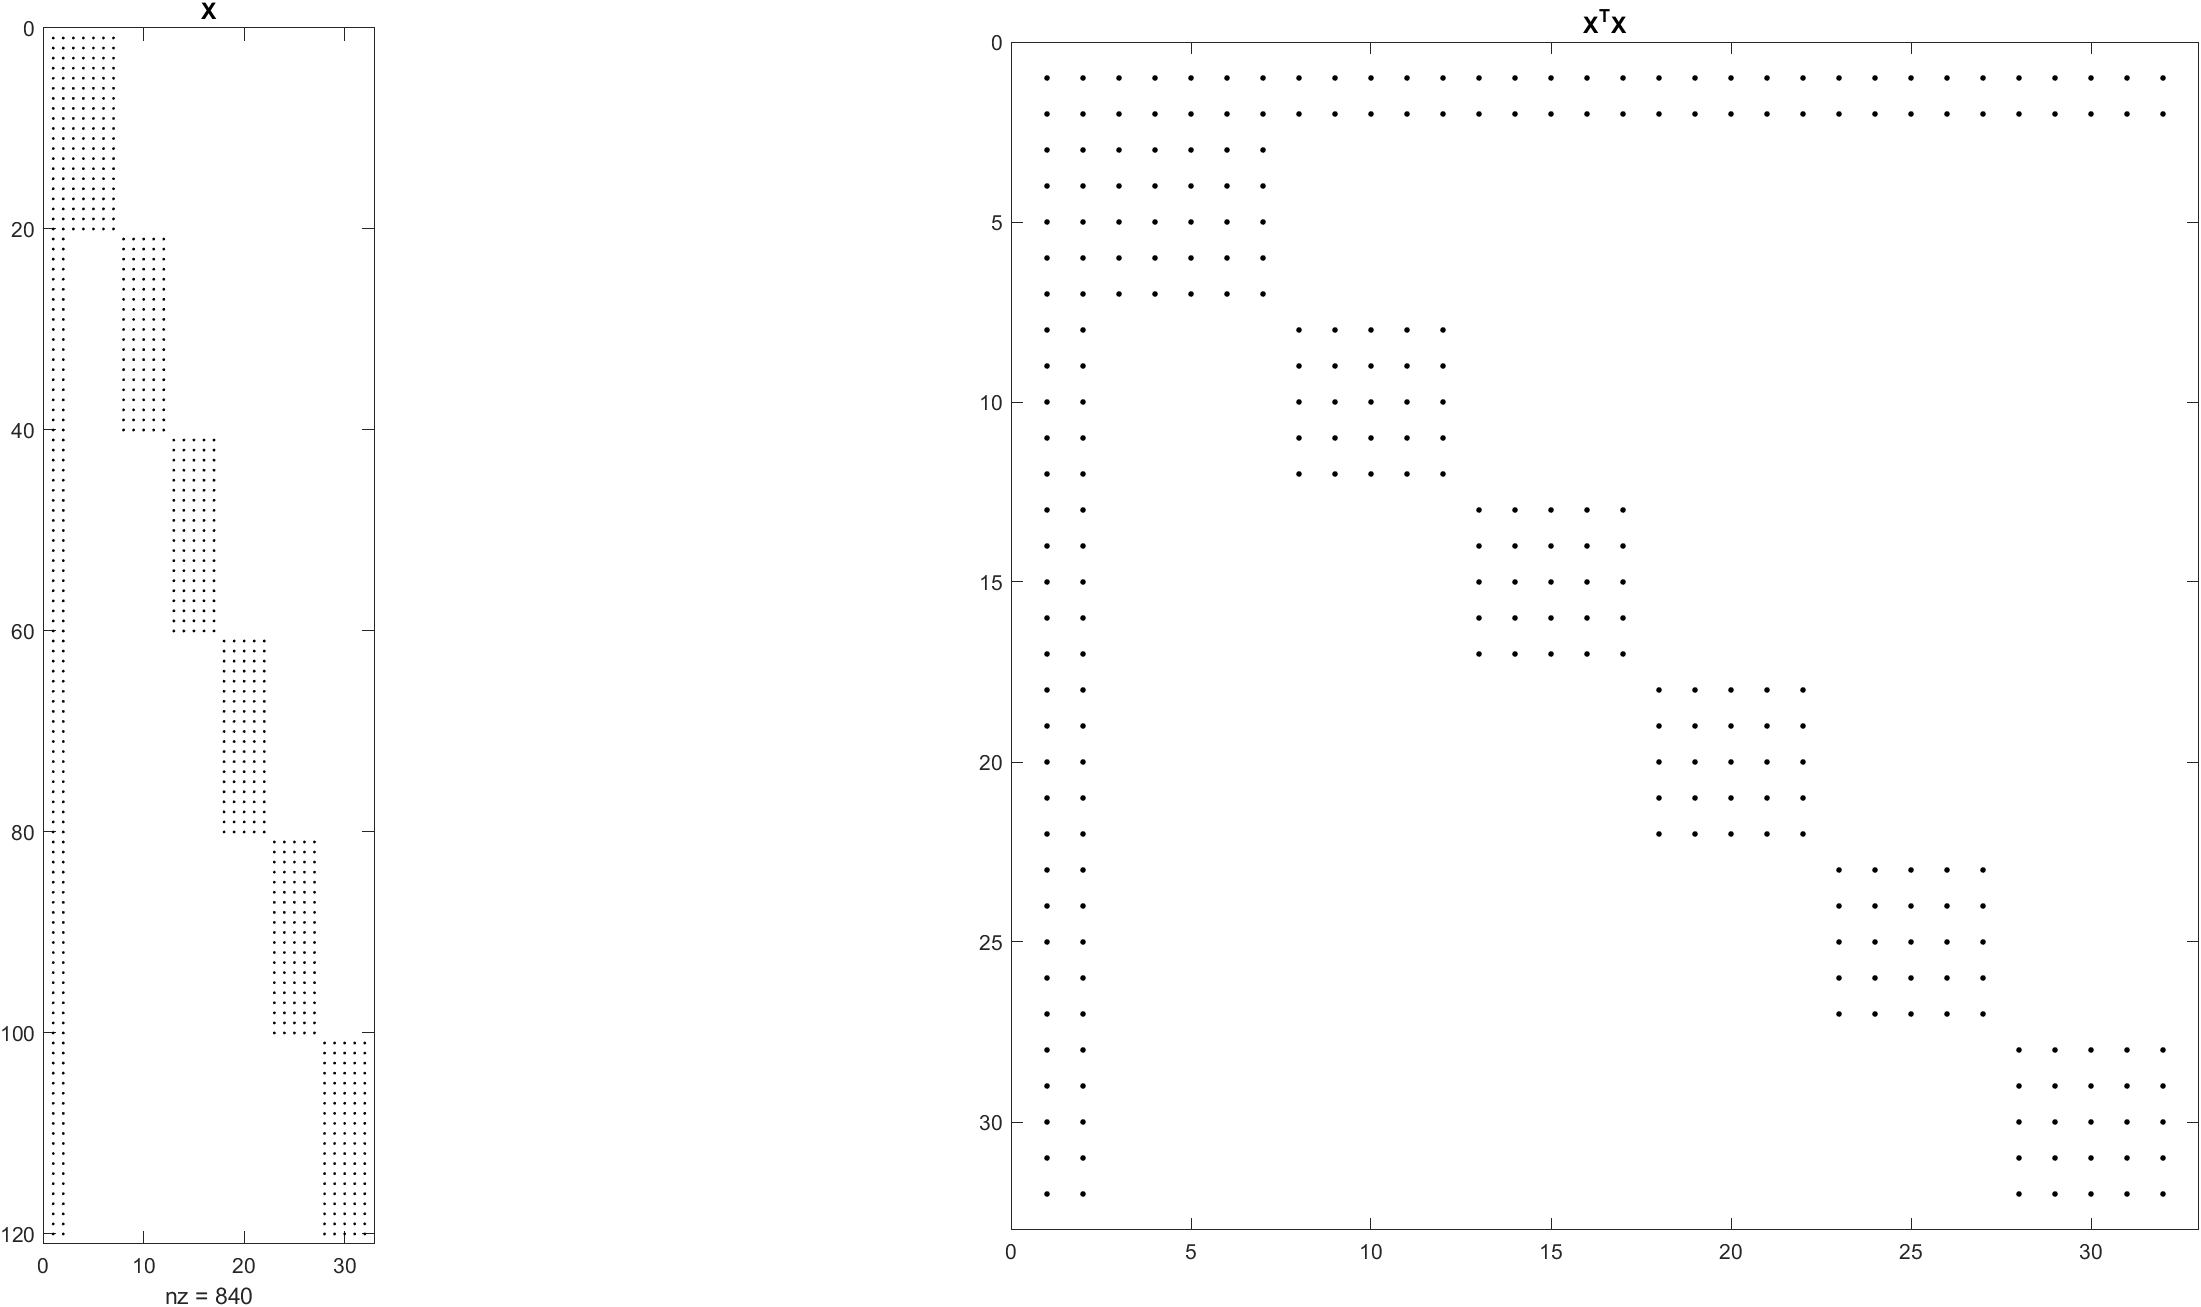
\includegraphics[width=\textwidth]{images/pattern_x.png}
	\centering
	\caption{\textit{On the left, sparsity pattern of an arbitrary matrix X as defined in \ref{matrix:x}.
			On the right, correspondent pattern of symmetric matrix $X^TX$.
			Inverse of this matrix is in general dense but does not get computed
			due to the high condition number of $X^TX$.}}
	\label{fig:pattern1}
\end{figure}
Notice that matrix $X^TX$ exhibits the pattern in
figure~\ref{fig:pattern1}, but as it happens with the normal equations, in
general this type of matrices have large condition number. An ......
factorization is stored in our implementation for performing several times this
matrix multiplication.

Define also the vector of coefficients $\bm{\nu} = (\bm{\beta}^\prime,
	\bm{b}_1^\prime, \dots, \bm{b}_m^\prime) \in \R^{mp+q-p}$.\\ Given these
definitions, we can write the mixed-effects model in \textit{implementation}
version with the formula
\begin{equation}
	\label{modelX}
	\bm{z} = X \bm{\nu} + \bm{f}_N + \bm{\epsilon},
\end{equation}
which separates the two components of our model, the parametric one
and the nonparametric. The estimation functional \ref{functional} can then be
expressed as
\begin{equation}
	\label{functional_short}
	J_{\Omega_i, \lambda} \left(\bm{\nu} , f_1, \dots, f_m \right) =
	\norm{\bm{z}-X\bm{\nu}  -\bm{f}_N}^2 + \lambda \sum_{i = 1}^m \int_{\Omega_i}\Delta f_i \left(\bm{p}\right)^2 d\Omega_i ,
\end{equation}
Next section describes the properties of a possible minimizer
$\left(\hat{\bm{\nu}} , \hat{f}_1, \dots, \hat{f}_m \right)$ of functional
\ref{functional_short}.
\section{Characterization of the solution}
Assuming that for each unit $i$, spatial field $f_i$ belongs to
$\mathcal{H}^2(\Omega_i)$, Sobolev space of functions whose first and second
derivative are in $\mathcal{L}^2(\Omega_i)$, the functional
\ref{functional_short} is well-defined.\\ We also make the assumption, not
strictly necessary, of imposing on every field $f_i$ homogeneous boundary
condition of Neumann type, meaning the normal derivative on the boundary is
null almost everywhere. Interesting applications of different type of boundary
conditions in the context of SR-PDE models are treated in \cite{Azzimonti}.

The field $f= \left(f_1 \dots f_m \right) $ is therefore naturally set in the
Hilbert space
\begin{equation}
	\mathcal{V}=\bigoplus_{i=1}^m \mathcal{H}^2_{n0}(\Omega_i)
\end{equation}
where $\mathcal{H}^2_{n0}(\Omega_i)$ is the set $\left\{g \in
	\mathcal{H}^2(\Omega_i) \mid \nabla g \cdot \bm{n} = 0 \text{ a.e. on } \partial \Omega_i\right\}$.

For the estimation problem introduced before, it holds the following:
\begin{theorem}
	With $\bm{\nu} \in \R^{mp+q-p}$ and $f =\left(f_1 \dots f_m \right) \in \mathcal{V}$, for functional $J_{\Omega_i, \lambda} \left(\bm{\nu} , f\right)$  there exists one and only one minimizer $\left(\hat{\bm{\nu}} , \hat{f} \right)$.
\end{theorem}

By denoting also with $\bm{\varphi}_N$ the vector obtained by concatenation of
the evaluations of a generic element $\varphi$ belonging to functional space
$\mathcal{V}$, at locations $n_i$ for every $i$, we have the following
characterization for the solution $\left(\hat{\bm{\nu}} , \hat{f} \right) =
	\left(\hat{\bm{\nu}} , \hat{f}_1, \dots, \hat{f}_m \right)$ of the estimation
problem:
\begin{equation}
	\begin{cases}
		\bm{\varphi}_N^T Q \hat{\bm{f}}_N + \lambda \sum_{i = 1}^m \int_{\Omega_i}\Delta \varphi_i \Delta \hat{f}_i  d\Omega_i = \bm{\varphi}_N^T Q \bm{z} \quad \forall \varphi \in \mathcal{V} \\
		\hat{\bm{\nu}}=\left(X^TX\right)^{-1}X^T(\bm{z}-\hat{\bm{f}}_N)
	\end{cases}
	. \label{sys1}
\end{equation}
First of previous equations can be equivalently rewritten into two
equations. With the introduction of an auxiliary function $\hat{g}$, whose
vector components are $-\Delta \hat{f}_i$, we write system \ref{sys1} as
\begin{equation}
	\label{triple}
	\begin{cases}
		\bm{\varphi}_N^T Q \hat{\bm{f}}_N + \lambda \sum_{i = 1}^m \int_{\Omega_i}\nabla \varphi_i \nabla g_i d\Omega_i = \bm{\varphi}_N^T Q \bm{z} \\
		\sum_{i=1}^{m}\left(\int_{\Omega_i}\eta_i \hat{g}_i d\Omega_i -\int_{\Omega_i}\nabla \eta_i \cdot \nabla \hat{f}_i d\Omega_i\right)=0       \\
		\hat{\bm{\nu}}=\left(X^TX\right)^{-1}X^T(\bm{z}-\hat{\bm{f}}_N)
	\end{cases}
	,
\end{equation}
valid for every couple $(\varphi,\eta)$ belonging to appropriate
functional spaces (essentially, we can work here with Sobolev spaces of degree
one).\\ This form of the problem is the most suitable for the use of the finite
element method to compute the desired estimation.

\section{Numerical solution}
\label{solution}
In the library \texttt{fdaPDE} we solve the estimation problem by mean of
finite elements (for detailed description see e.g. \cite{quarteronitosto}). We
generate a triangular mesh, by partitioning domains $\Omega_i$ with a regular
triangulation. Domain $\Omega_i$ is therefore approximated as
$\Omega_i^{\tau_i}$, union of the triangles.

On the approximated domains we define Sobolev spaces,
$\mathcal{H}^1_i\left(\Omega_i^{\tau_i}\right)$, for every $i$, and relative
subspaces, $\mathcal{V}^1_{i}\left(\Omega_i^{\tau_i}\right)$, \ie the finite
element space of degree one on triangulation $\tau_i$: in this work we will
limit ourselves to Lagrangian finite elements of degree one with nodes in the
vertices of the triangles.

Having defined this spaces, we move to the discrete counterpart of problem
\ref{triple}. The equations remain the same if not for the domain $\Omega_i$ ,
approximated as $\Omega_i^{\tau_i}$. But as we change functional spaces from
infinite dimension to finite dimension:
\begin{itemize}
	%	\item
	%	      \listvalues
	\item[--] we can write functions as linear (finite) combinations of finite
		element basis; we denote as $\bm{\psi}_i$ or $\bm{\psi}^{\left(i\right)}$ if
		necessary, the vector of fields that constitute a basis for
		$\mathcal{V}^1_{i}\left(\Omega_i^{\tau_i}\right)$;
	\item[--] we can compute integrals by
		numerical techniques, see \cite{quarteronitosto} for technical
		details;
	\item[--] thanks to previous two points, problem \ref{triple} is
		equivalently written in algebraic form as a linear system of equations.
\end{itemize}
The following matrices definitions are used:
\begin{equation}
	\label{Psi_i}
	\Psi_i=
	\begin{bmatrix}
		\psi_1^{(i)}\left(\bm{p}_{i1}\right)   & \ldots & \psi_{N_{\tau_i}}^{(i)}\left(\bm{p}_{i1}\right)   \\
		\vdots                                 & \ddots & \vdots                                            \\
		\psi_1^{(i)}\left(\bm{p}_{in_i}\right) & \ldots & \psi_{N_{\tau_i}}^{(i)}\left(\bm{p}_{in_i}\right)
	\end{bmatrix}
	.
\end{equation}
$\Psi_i$ belongs to $\R^{n_i \times N_{\tau_i}}$, where we define
$N_{\tau_i}$ as the number of basis functions deriving from triangulation
$\tau_i$ relative to $\Omega_i$. Given Neumann boundary conditions, this is
also the number of nodes of the $i$-th mesh.
\begin{equation}
	R_{0i}=\int_{\Omega_{\tau_i}} \bm{\psi}_i \bm{\psi}^T_i d\Omega_{\tau_i}.
\end{equation}
$R_{0i}$ lies in $\R^{N_{\tau_i} \times N_{\tau_i}}$.
\begin{equation}
	R_{1i}=\int_{\Omega_{\tau_i}} \left( \nabla \bm{\psi}_i\right)^T \nabla  \bm{\psi}_i d\Omega_{\tau_i}.
\end{equation}
$R_{1i}$ lies in $\R^{N_{\tau_i} \times N_{\tau_i}}$ as well, with
$\nabla \bm{\psi}_i$ being the matrix whose element in $m$-th row and $n$-th
column is $\pdev{\left(\bm{\psi}_i\right)_n}{x_m}$.

Before we used the operator mapping a generic element $\varphi$, belonging to
functional space $\mathcal{V}$, to $\bm{\varphi}_N$, the vector obtained by
concatenation of the evaluations of $\varphi$, at locations $n_i$ for every
$i$. Define $N_{\tau}= \sum_{i=1}^{m} N_{\tau_i}$ the total number of degrees
of freedom for all the statistical units. By defining $\tilde{\Psi}$, $\in
	\R^{N \times N_{\tau}}$ as
\begin{equation}
	\label{Psitilde}
	\tilde{\Psi}=
	\begin{bmatrix}
		\Psi_1 &        & 0      \\
		       & \ddots &        \\
		0      &        & \Psi_m
	\end{bmatrix}
	,
\end{equation}
the following identity shows the role of $\Psi_i$ matrices:
\begin{equation}
	\bm{\varphi}_N=\tilde{\Psi}\bm{\varphi}
\end{equation}
where $\bm{\varphi}$ is the coefficient vector of expansion of
$\varphi$ with respect to the considered finite element basis.

Analogously as $\tilde{\Psi}$, we define the tensorised versions of $R_0$ and
$R_1$ ($\in \R^{N_{\tau} \times N_{\tau}}$) matrices as:
\begin{equation}
	\tilde{R_0}=
	\begin{bmatrix}
		R_{01} &        & 0      \\
		       & \ddots &        \\
		0      &        & R_{0m}
	\end{bmatrix}
	,
\end{equation}
\begin{equation}
	\tilde{R_1}=
	\begin{bmatrix}
		R_{11} &        & 0      \\
		       & \ddots &        \\
		0      &        & R_{1m}
	\end{bmatrix}
	.
\end{equation}

By mean of simple algebraic manipulations, we express equivalently the discrete
counterpart of problem \ref{triple} with the following linear system of
equations:

\begin{equation}
	\label{mono}
	\begin{bmatrix}
		\tilde{\Psi}^TQ\tilde{\Psi} & -\lambda \tilde{R}_1^T \\
		-\lambda \tilde{R}_1        & -\lambda \tilde{R}_0
	\end{bmatrix}
	\begin{bmatrix}
		\hat{\bm{f}} \\
		\hat{\bm{g}}
	\end{bmatrix}
	=
	\begin{bmatrix}
		\tilde{\Psi}^T Q\bm{z} \\
		0
	\end{bmatrix}
\end{equation}
together with the least square equation for parameter $\bm{\nu}$,
which can be rewritten as
\begin{equation}
	\label{nu}
	\hat{\bm{\nu}}=\left(X^TX\right)^{-1}X^T(\bm{z}-\tilde{\Psi}\hat{\bm{f}})
\end{equation}
System \ref{mono} has dimensions $\left(2 N_{\tau}\right)^2$. We call
system \ref{mono} monolithic because it might be tough to solve it by standard
numerical techniques. In fact $N_{\tau}$ might be large, for both the presence
of a large number of statistical units $m$ or thanks to a large number of nodes
$N_{\tau_i}$ for each unit.

Therefore, aim of this work is to avoid the solution of such high dimension
linear system, in favour of splitting it into many systems ($m$) of lower
dimension.

In case the dimensions of the monolithic system are treatable, the Woodbury
decomposition formula, described in appendix \ref{sec:wood}, can be used to
speed up the computation of the solution for different values of $\lambda$. The
decomposition for system \ref{mono} is analogous to the one described in the
appendix, with
\begin{equation}
	\label{eq:wootilde}
	E =
	\begin{bmatrix}
		\tilde{\Psi}^T\tilde{\Psi} & -\lambda \tilde{R}_1^T \\
		-\lambda \tilde{R}_1       & -\lambda \tilde{R}_0
	\end{bmatrix}
	\quad U =
	\begin{bmatrix}
		\tilde{\Psi}^TX \\
		0
	\end{bmatrix}
\end{equation}
\begin{equation*}
	C = -
	\begin{bmatrix}
		\left(X^TX\right)^{-1}
	\end{bmatrix}
	\quad V = U^T;
\end{equation*} again, despite $E$ being of same dimension as the monolithic system,
it has the property of being fully sparse.

This was the approach used by \citeauthor{kim} in her work \cite{kim}. The
monolithic system, as data was coming from hundreds of units, quickly failed to
scale at such dimension. In next section we present an iterative method that,
under some hypothesis discussed in section \ref{assumptions}, does not require
storing matrices such as $\tilde{R}_0$, $\tilde{R}_1$, $\tilde{\Psi}$. Despite
this hypothesis being quite restrictive, for example the domain $\Omega_i$
being the same across units, in many applications they can be relaxed. As an
example, when applying this model on brain data, we will see in chapter
\ref{ch:Applications} that different brain surfaces for each patient get
approximated as a common standardized surface, making the iterative method
particularly effective.
